\chapter{مقایسه، آزمایش‌ها، و نتایج}
در این فصل به بررسی نتایج حاصل از پیاده‌سازی الگوریتم‌ها و مقایسه آن‌ها می‌پردازیم.
\section{فرآیند آزمایش}
برای آزمایش، ابتدا الگوریتم‌های معرفی‌ شده در فصل‌های قبل را با یک میلیون گام علیه دروازه‌بان کد پایه ایجنت
آموزش می‌دهیم، و نمودار‌های فرآیند یادگیری را بررسی می‌کنیم. در هر ۵۰۰۰ گام از آموزش مدل به صورت تناوبی ذخیره می‌شود، و در نهایت بهترین مدل‌ها را انتخاب می‌کنیم.
لازم به ذکر است که منظور از گام، گام‌های یادگیری تقویتی است، که هرکدام متناظر با یک ضربه به توپ اند و منظور گام‌های شبیه‌ساز فوتبال نیست.

در نهایت مدل انتخاب شده را برای ۱۰۰ ضربه پنالتی علیه کد پایه قرار می‌دهیم تا با سیاست حریصانه و بدون تصمیم‌گیری تصادفی سنجیده شود، و درصد وقوع هر یک از حالت‌های پایانی بازی را بررسی می‌کنیم.
در نهایت راهکار‌های متفاوتی را برای بهبود نتایج یادگیری امتحان می‌کنیم.

تمامی آزمایش‌ها روی یک سیستم با پردازنده‌ی \lr{AMD Ryzen 7 6800H}، 
حافظه ۳۲ گیگابایت،
و کارت گرافیک \lr{NVIDIA RTX 3070Ti} انجام شده است، 
همراه‌ با کتاب‌خانه‌های کودا 
\LTRfootnote{CUDA}
\lr{CUDA 12.4}, \lr{cudnn 8.9.2}، و \lr{cublas 12.1.3}
انجام شده‌است.
\section{ارزیابی الگوریتم‌ها}
در ابتدا الگوریتم \lr{DQN} را برای یادگیری از صفر امتحان می‌کنیم.
بعد از یک میلیون گام آموزش که حدود ۱۲ ساعت طول کشید، عامل موفق به کشف تکنیک گل زدن نشد.
فرآیند آموزش ۵ بار و با ابرپارامتر‌های متفاوت آزمایش شد؛ اما در هیچ یک از اجرا‌ها عامل موفق به یادگیری نشد.
یکی از دلایل ممکن این موضوع می‌تواند تفاوت زیاد بین پاداش‌های موفق و ناموفق باشد؛ چرا که این موضوع ابعاد گرادیان را بزرگ کرده و باعث عدم ثبات می‌شود. به همین منظور یک ضریب مقیاس‌گر 
برای پاداش‌ها اضافه شد، که باز هم موثر در موفقیت نبود.

\begin{figure}[H]
    \centering
    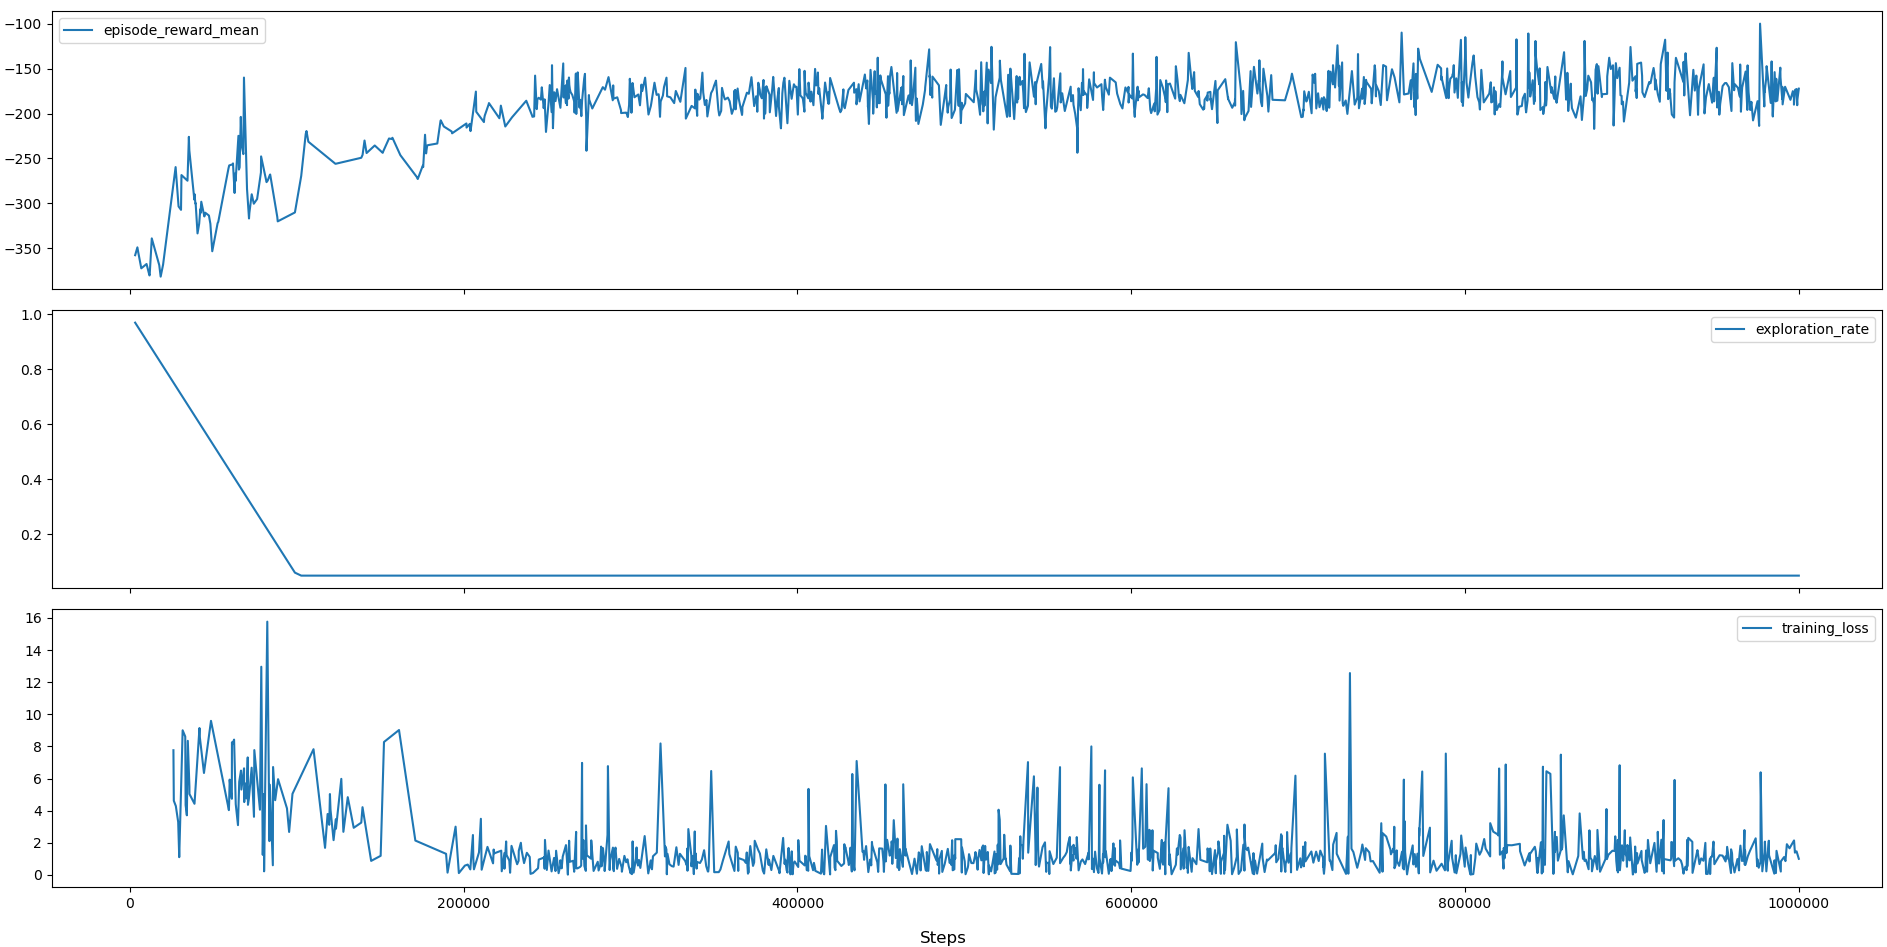
\includegraphics[width=1\textwidth]{images/DQN_graphs.png}
    \caption{نمودار سه پارامتر متفاوت برای یک اجرای الگوریتم \lr{DQN}}\label{fig:dqn_graphs}
\end{figure}

در شکل \ref{fig:dqn_graphs}
می‌توان به ترتیب میانگین پاداش عامل، نرخ کاوش، و خطای شبکه عصبی را در طی زمان آموزش دید.
محور افقی این نمودار گام‌های آموزش است، که در اینجا ۱ میلیون گام است.
مقیاس پاداش‌ها برای این اجرا، ۰.۲
بوده‌است و برای رسم نمودار، به مقیاس ۱ تبدیل شده‌است.
همانطور که می‌توان مشاهده کرد، نمودار خطای شبکه از گام ۵۰۰۰۰ آغاز شده. این به این علت است که آموزش شبکه از این گام آغاز می‌شود؛ تا پیش از آن بافر با حالت‌های متفاوت پر شود.

همانطور که قابل مشاهده است، پاداش‌ها نسبت به حالت آغازین افزایش می‌یابند اما عامل موفق به کشف حالت گل زدن نشده‌است.
میزان خطای شبکه عصبی نیز در طول زمان کاهش یافته و نزدیک به ۱ شده، اما این هم نشان‌دهنده‌ی یادگیری موفق نیست، بلکه شبکه همواره (به درستی)
میزان ارزش حالت شکست را خروجی می‌دهد.

همین فرآیند را با الگوریتم \lr{DDPG} تکرار می‌کنیم.
می‌توان مشاهده کرد که عامل در زیر ۱۰۰ هزار گام موفق به کشف تکنیک گل زدن شده‌است.
همچنین همانطور که در فصل‌های قبلی ذکر شد، به علت محدود بودن اندازه بافر، عامل ممکن است یادگیری خود را فراموش کند.

\begin{figure}[H]
    \centering
    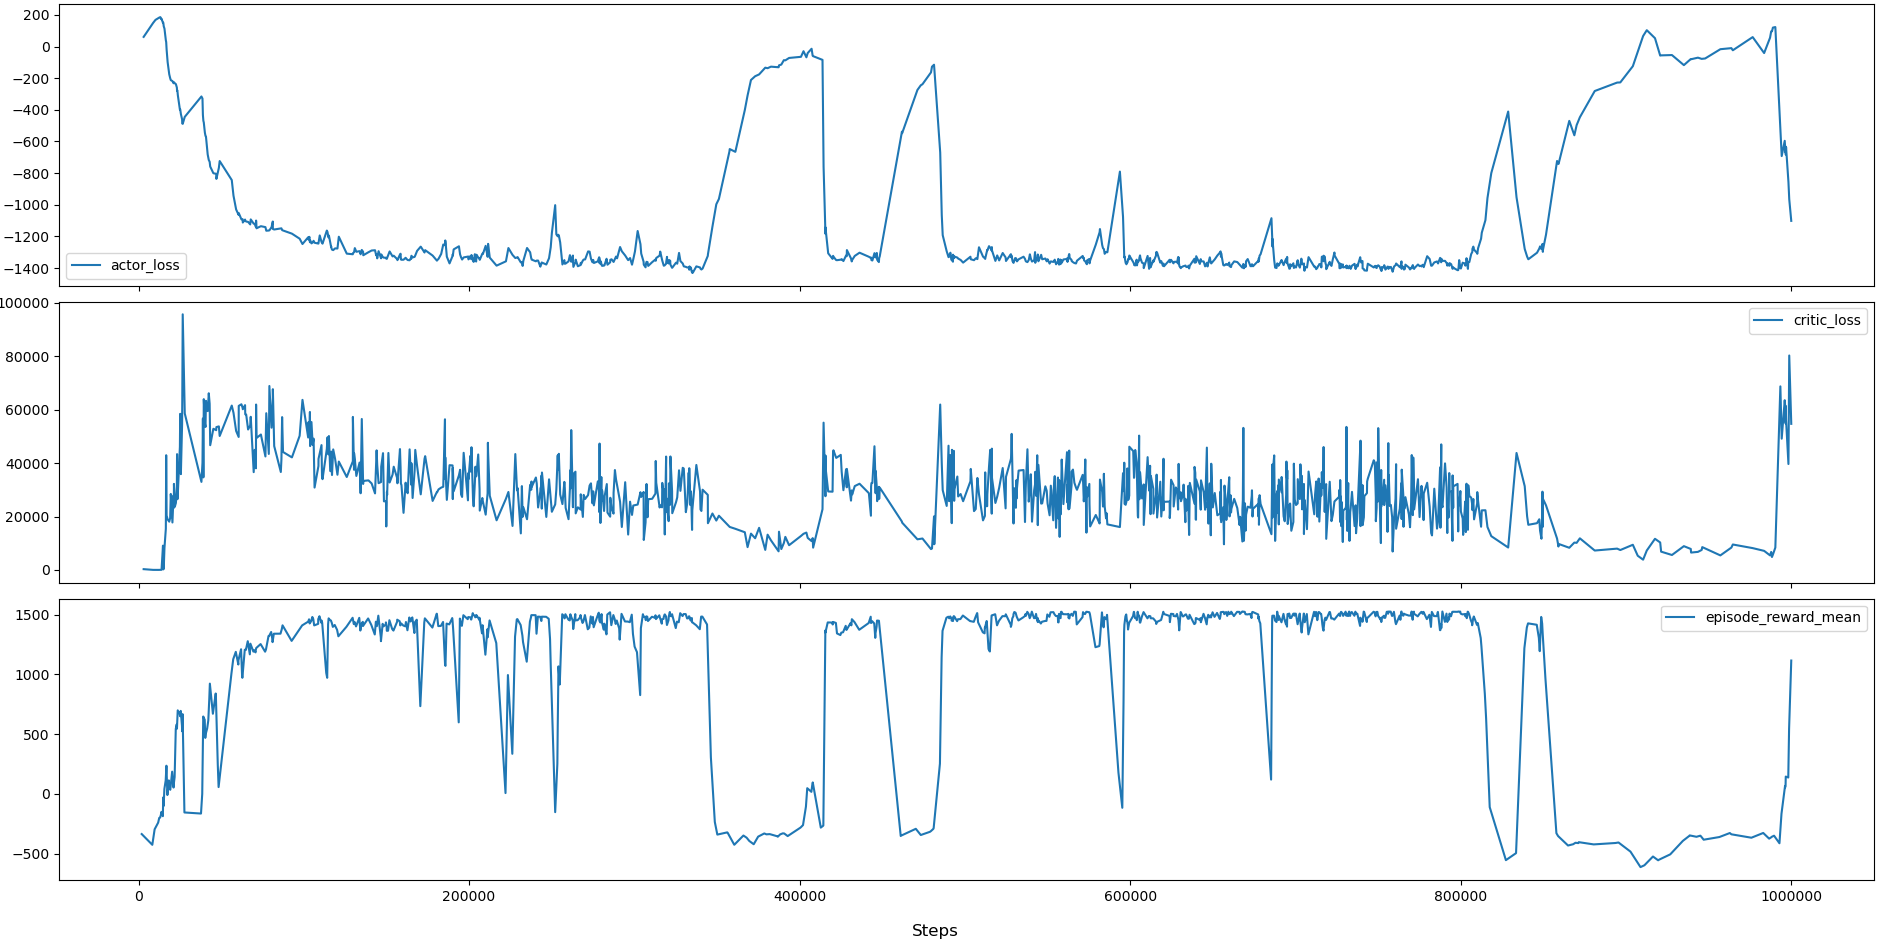
\includegraphics[width=1\textwidth]{images/DDPG_graphs.png}
    \caption{نمودار سه پارامتر متفاوت برای یک اجرای الگوریتم \lr{DDPG}}\label{fig:ddpg_graphs}
\end{figure}

در شکل \ref{fig:ddpg_graphs}
می‌توان به ترتیب خطای شبکه بازیگر، خطای شبکه نقاد، و میانگین پاداش عامل را در طی زمان آموزش دید.
همانطور که مشاهده می‌شود، در حین موفقیت عامل، خطای شبکه‌ها و به ویژه خطای بازیگر کاهش یافته است.

\begin{table}[H]
    \centering
    \caption{بهترین نتایج الگوریتم‌ها مقابل کد پایه ایجنت برای صد پنالتی.}
    \begin{tabular}{ |p{4cm}|p{2cm}|p{2cm}|  }
        \hline
        خروجی & \lr{DQN} & \lr{DDPG} \\
        \hline
        گل زدن & ۲ & ۹۹\\
        \hline
        بیرون رفتن توپ & ۱۸ & ۰\\
        \hline
        گرفتن توسط دروازه‌بان & ۷۴ & ۱\\
        \hline
        اتمام زمان & ۶ & ۰\\
        \hline
        \end{tabular}
        \label{tab:base_results}
\end{table}

با توجه به اینکه الگوریتم \lr{DDPG} موفق بود، می‌توان حدس‌هایی راجع به عدم موفقیت \lr{DQN} زد.
یکی از دلایل، این است که به علت گسسته بودن اعمال، تعداد گام‌های لازم برای رسیدن به گل بیشتر است، و از آنجا که عامل باید به صورت تصادفی گل زدن را کشف کند،
عامل به تعداد دفعات کافی به این حالت نمی‌رسد.
همچنین همانطور که در شکل \ref{fig:actor_critic} می‌توان دید، شبکه در الگوریتم
\lr{DQN} به ازای هر عمل، یک خروجی دارد و به همین علت، فضای عمل بزرگ یادگیری را به مراتب دشوار می‌کند.
از این رو می‌توان سه راه را برای بهبود یادگیری این الگوریتم پیشنهاد داد:
\begin{enumerate}
    \item بهبود گسسته‌سازی عمل‌ها.
    \item استفاده از پاداش‌های بهتر برای حالت‌های غیرنهایی که عامل را به سمت حالت‌های مفید‌تر هدایت کند.
    \item تغییر فضای عمل و جدا‌سازی اعمال به دریبل‌ زدن و شوت زدن.
\end{enumerate}

\section{بهبود تابع پاداش}
برای بهبود تابع پاداش، به روش گل‌زنی الگوریتم \lr{DDPG} نگاه می‌کنیم.
به نظر می‌آید که نزدیک شدن دروازه‌بان به توپ عامل منفی‌ای نیست؛ چرا که این حالت ممکن است به عامل کمک کند تا با یک ضربه به توپ، زاویه دروازه را باز کند.
همچنین در صورت نزدیکی بیش از حد دروازه‌بان به توپ در حین ضربه، عامل می‌تواند از قابلیت گسسته بودن زمان شبیه‌ساز استفاده کند و با انجام قوی‌ترین ضربه ممکن، توپ را از روی دروازه‌بان بگذراند.
بنابرین برای گام‌های بعدی، عامل فاصله با دروازه‌بان را از محاسبات پاداش حذف می‌کنیم.


\section{جدا‌سازی عمل شوت}
عامل در ابتدای یادگیری، هنوز به درک اینکه در چه حالتی می‌تواند شوت منجر به گل داشته باشد نرسیده است.
از آنجا که این عمل با عمل رسیدن به موقعیت شوت‌زنی متفاوت است، عامل ممکن است دیر به دیر به حالت‌هایی که شوت زدن در آن ممکن است برسد.
بنابرین در حین یادگیری نسبت به ضربه با سرعت‌های بالا بدبین می‌شود.

برای حل این مشکل، فضای عمل را به گونه‌ای اصلاح می‌کنیم که شوت زدن جدا باشد.
\subsection{شوت با رفتار سطح بالای کد پایه}
یک عمل خاص مدنظر می‌گیریم که در صورت انتخاب شدن توسط عامل، شوت کد پایه ایجنت
انجام می‌شود. این کد در صورت وجود شوت ممکن، آن را انجام می‌دهد و در غیر این صورت، هیچ عملی انجام نمی‌شود.
در صورتی که عامل این عمل را انتخاب کند ولی به گل نرسد، پاداش منفی‌ای به آن داده می‌شود، تا عامل استفاده صحیح از این ابزار را یاد بگیرد.
\begin{figure}[H]
    \centering
    \begin{tikzpicture}
        \pie[rotate=90, color={green, red, orange, yellow}]
        {
            3/گل,
            12/توپ رفتن بیرون,
            49/دروازه‌بان توسط گرفتن,
            36/زمان اتمام
        }
    \end{tikzpicture}
    \caption{نتیجه ۱۰۰ ضربه پنالتی با شوت سطح بالا مقابل کد پایه ایجنت برای عامل یادگیری‌شده}\label{fig:helios_shoot_pie}
\end{figure}

طبق تجربه پیش از این پروژه، این رفتار سطح بالا بسیار محافظ‌کارانه تصمیم می‌گیرد.
از این رو شاید کمک چندانی به عامل برای یادگیری نکند.
همچنین از آنجا که استفاده از این قابلیت بسیار وابسته به شبیه‌سازی ضربه به توپ و بررسی امکان قطع توپ توسط دروازه‌بان است، خلاف ماهیت انجام این پروژه است.
\subsection{عمل شوت به نقاط ثابت دروازه}
فرض کنید تعدادی نقطه ثابت دروازه را انتخاب کنیم.
هر یک از این نقاط متناظر با یک عمل شوت است.
در این عمل، به توپ با حداکثر سرعت ممکن در راستای این عمل ضربه می‌زنیم.
برای انتخاب نقاط، دو تیرک دروازه را به عنوان نقاط ثابت در نظر گرفته، و فضای بین این نقطه را به $n-1$ نقطه تقسیم می‌کنیم.
\begin{figure}[H]
    \centering
    \begin{tikzpicture}
        \pie[rotate=90, color={green, red, orange, yellow}]
        {
            19/گل,
            4/توپ رفتن بیرون,
            53/دروازه‌بان توسط گرفتن,
            24/زمان اتمام
        }
    \end{tikzpicture}
    \caption{نتیجه تست ۱۰۰ پنالتی مقابل کد پایه ایجنت با ۵ نقطه شوت}\label{fig:custom_shoot_pie}
\end{figure}

\section{تغییر گسسته‌سازی}
حال که عامل دارای عمل مستقیم شوت است، می‌توانیم گسسته‌سازی قدرت را به گونه‌ای تغییر دهیم که سرعت‌های بالا را نداشته باشد.
برای این منظور ضربه به توپ را به سه سرعت تقسیم می‌کنیم: ۱۵ درصد حداکثر سرعت توپ، ۲۵ درصد حداکثر سرعت توپ، و ۵۰ درصد حداکثر سرعت توپ.
در واقع اعمال ممکن را به شوت به نقطه یا دریبل با سرعت و زاویه معین تقسیم می‌کنیم.

همچنین به صورت شهودی می‌توان برداشت کرد که تقسیم زوایای جلوی بازیکن به شدت مهم‌تر از زوایای پشت بازیکن است، 
چرا که به ندرت نیاز می‌شود بازیکن با ضربه به عقب پیشرفت کند.
زوایای جلوی بازیکن را به ۹ قسمت تقسیم می‌کنیم، و دو راستا برای دریبل به عقب (بالا عقب و پایین عقب) اضافه می‌کنیم.

با ترکیب این دو تکنیک، فضای حالت از ۱۲۰ عمل، به ۳۸ عمل کاهش می‌یابد.
این کاهش از دو راستا به یادگیری ما کمک می‌کند:
\begin{itemize}
    \item کاهش ابعاد گرادیان و افزایش سرعت یادگیری
    \item افزایش احتمال انجام عمل مفید به کمک کاوش، به علت حذف رفتار‌هایی که به احتمال زیاد مفید نیستند
\end{itemize}
پس از یک میلیون گام آموزش، نمودار پاداش‌ها و درصد موفقیت در حین آموزش را مشاهده می‌کنیم.
\begin{figure}[H]
    \centering
    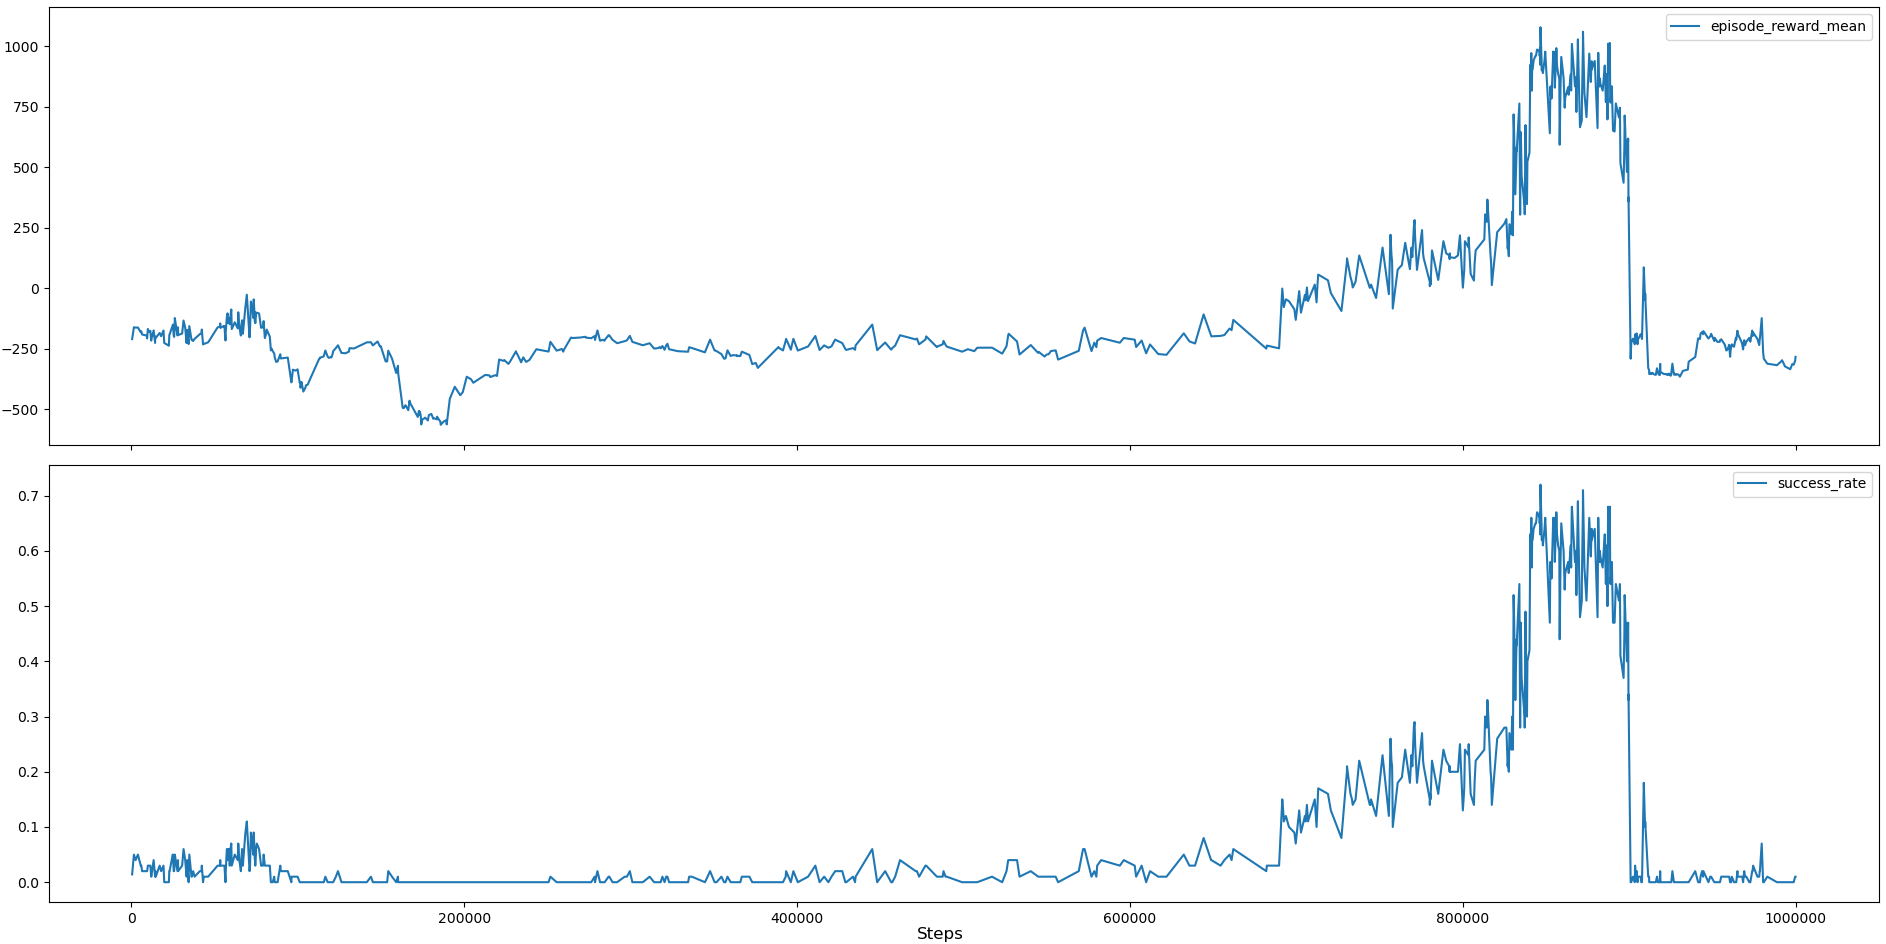
\includegraphics[width=1\textwidth]{images/dqn_discretization.png}
    \caption{نمودار میانگین پاداش و میانگین نرخ گل‌زنی \lr{DQN} با تغییرات گسسته‌سازی}\label{fig:discretization_change}
\end{figure}
همانطور که در تصویر مشاهده می‌کنید، با این تغییرات عامل موفق به کشف روش گل‌زنی و موفقیت ۷۲ درصد در حین آموزش شده‌است.
همچنین می‌توان دید که نمودار پاداش و نرخ گل‌زنی هم‌رفتار و تقریبا هم‌شکل هستند.
\begin{figure}[H]
    \centering
    \begin{tikzpicture}
        \pie[rotate=90, color={green, red, orange, yellow}]
        {
            74/گل,
            2/توپ رفتن بیرون,
            24/دروازه‌بان توسط گرفتن,
            0/زمان اتمام
        }
    \end{tikzpicture}
    \caption{نتیجه تست ۱۰۰ پنالتی مقابل کد پایه ایجنت با بهبود روش گسسته‌سازی}\label{fig:discretization_pie}
\end{figure}

\section{بررسی تعمیم پذیری}
در این بخش، با تست علیه دروازه‌بان تیم‌هایی که مقابل آن‌ها یادگیری رخ نداده، می‌بینیم که آیا این یادگیری تعمیم‌پذیر بوده یا خیر.
با توجه به اینکه پس از مسابقات، فایل‌های اجرایی تیم‌ها در اختیار سایر شرکت‌کنندگان قرار می‌گیرد، می‌توانیم این تست را انجام دهیم.
از ۳ تیم برای این منظور استفاده می‌کنیم:
نسخه ۲۰۲۳ تیم 
هلیوس\LTRfootnote{Helios2023}
 که قهرمان پیاپی چندین دوره مسابقات است، تیم کد پایه ایجنت
 که مبنای بسیاری از سایر تیم‌ها است،
و نسخه ۲۰۲۳ تیم یوشان\LTRfootnote{YuShan2023}
 که از تیم‌های موفق دیگر است و استراتژی متفاوتی نسبت به دو تیم قبلی دارد.

\begin{table}[H]
    \centering
    \caption{نتایج تست الگوریتم \lr{DDPG} علیه تیم‌های مختلف}\label{tab:generalization}
    \begin{tabular}{ |p{4cm}|p{3cm}|p{3cm}|p{3cm}|  }
            \hline
            خروجی & ایجنت & هلیوس ۲۰۲۳ & یوشان ۲۰۲۳\\
            \hline
            گل زدن & ۹۹ & ۴۰ & ۲۷ \\
            \hline
            بیرون رفتن توپ & ۰ &۴ & ۱۱ \\
            \hline
            گرفتن توسط دروازه‌بان & ۱ &۴۰ & ۵۷ \\
            \hline
            اتمام زمان & ۰ &۱۶ & ۴ \\
            \hline
        \end{tabular}
\end{table}
به صورت شهودی و با دیدن نتایج تست، می‌توان پی برد که نتایج تا حدودی قابل تعمیم است، اما شوت زدن عامل بسیار وابسته به مختصات دروازه‌بان است و از این رو، شوت‌های به بیرون و یا گرفته شده توسط دروازه‌بان افزایش یافته‌اند.
همچنین دروازه‌بان سایر تیم‌ها مانند هلیوس،
 در شرایطی که نتوانند به توپ برسند از دستور تکل استفاده می‌کنند، که برد بیشتری نسبت به گرفتن توپ دارد ولی به صورت احتمالاتی است. در صورت تکل موفق حالت گرفتن توسط دروازه‌بان ثبت می‌شود.

\begin{table}[H]
    \centering
    \caption{نتایج تست الگوریتم \lr{DQN} بهبود یافته مقابل تیم‌های مختلف}\label{tab:dqn_generalization}
    \begin{tabular}{ |p{4cm}|p{3cm}|p{3cm}|p{3cm}|  }
            \hline
            خروجی & ایجنت & هلیوس ۲۰۲۳ & یوشان ۲۰۲۳\\
            \hline
            گل زدن & ۷۱ & ۰ & ۱۰ \\
            \hline
            بیرون رفتن توپ & ۰ &۰ & ۱۵ \\
            \hline
            گرفتن توسط دروازه‌بان & ۲۹ &۱۰۰ & ۷۰ \\
            \hline
            اتمام زمان & ۰ &۰ & ۵ \\
            \hline
        \end{tabular}
\end{table}
با توجه به گسسته‌سازی، هر گونه تغییر در موقعیت دروازه‌بان عمل بعدی عامل را به شدت تحت تاثیر قرار می‌دهد و عامل به شدت با حالت‌های از پیش دیده‌شده فاصله می‌گیرد.
از این رو همانطور که پیش‌بینی می‌شد، تعمیم‌پذیری این الگوریتم به تیم‌های دیگر بسیار پایین است.

در نهایت یادگیری الگوریتم \lr{DDPG} را تکرار می‌کنیم، با این تفاوت که آموزش را از ابتدا و مقابل تیم‌های مختلف انجام می‌دهیم.
این آزمایش از این رو است که ببینیم در صورتی که آموزش روی تیم‌های قوی‌تر انجام شود، آیا عامل موفق به یادگیری تکنیک‌های مفید‌تری می‌شود یا خیر.

فرآیند آموزش تا زمانی ادامه می‌یابد که عامل به تکنیک گل‌زنی مقابل تیم آموزشی برسد، و تا یک میلیون گام ادامه نخواهد یافت.
برای یادگیری مقابل تیم هلیوس فقط ۱۵۰ هزار گام کافی بود تا نرخ موفقیت به بالای ۹۰ درصد برسد که حدود یک ساعت زمان برد. یادگیری مقابل تیم یوشان حدود ۷۰ هزار گام طول کشید که ۲۰ دقیقه زمان برد.


\begin{table}[H]
    \centering
    \caption{نتایج تست الگوریتم \lr{DDPG} علیه تیم‌های مختلف با آموزش مقابل تیم هلیوس}\label{tab:ddpg_helios_generalization}
    \begin{tabular}{ |p{4cm}|p{3cm}|p{3cm}|p{3cm}|  }
            \hline
            خروجی & ایجنت & هلیوس ۲۰۲۳ & یوشان ۲۰۲۳\\
            \hline
            گل زدن & ۴۷ & ۹۰ & ۲۳ \\
            \hline
            بیرون رفتن توپ & ۱۶ &۰ & ۵ \\
            \hline
            گرفتن توسط دروازه‌بان & ۳۷ &۷ & ۶۵ \\
            \hline
            اتمام زمان & ۰ &۳ & ۷ \\
            \hline
        \end{tabular}
\end{table}

\begin{table}[H]
    \centering
    \caption{نتایج تست الگوریتم \lr{DDPG} علیه تیم‌های مختلف با آموزش مقابل تیم یوشان}\label{tab:ddpg_yushan_generalization}
        \begin{tabular}{ |p{4cm}|p{3cm}|p{3cm}|p{3cm}|  }
            \hline
            خروجی & ایجنت & هلیوس ۲۰۲۳ & یوشان ۲۰۲۳\\
            \hline
            گل زدن & ۰ & ۰ & ۹۹ \\
            \hline
            بیرون رفتن توپ & ۰ &۰ & ۰ \\
            \hline
            گرفتن توسط دروازه‌بان & ۸۳ &۱۰۰ & ۱ \\
            \hline
            اتمام زمان & ۱۷ &۰ & ۰ \\
            \hline
        \end{tabular}
\end{table}

به نظر می‌رسد که استراتژی متفاوت یوشان باعث می‌شود عامل‌هایی که روی سایر تیم‌ها آموزش دیده‌اند گیج شوند و نتوانند به موفقیت برسند.
اما آموزش روی یوشان که به دور زدن دروازه‌بان در آن آسان‌تر است، باعث می‌شود که عامل 
به موفقیت جلوی سایر تیم‌ها نرسد، چرا که تاکتیک موفق جلوی یوشان منجر به گرفتن توسط دروازه‌بان می‌شود.

از سوی دیگر، با توجه به این که استراتژی هلیوس مشابه ولی قوی‌تر نسبت به کد ایجنت است، آموزش مقابل آن باعث می‌شود که عامل به موفقیت نسبی نزدیک شود.

لازم به ذکر است که حتی اگر عامل در دو دور آموزش مقابل تیم آموزشی به نتایج یکسان برسد، نمی‌توان انتظار داشت که نتایج تست مقابل سایر تیم‌ها یکسان باشد. به این منظور که اگر آموزش را دو بار از صفر آغاز کنیم و تا صد درصد موفقیت پیش ببریم، ممکن است نتایج تست مقابل تیم‌های دیگر بین دو حالت نزدیک نباشد. از این رو این آزمایش معیار خیلی دقیقی برای بررسی کمی تعمیم‌پذیری نیست.

در آینده می‌توان راه‌های تولید مدل‌های تعمیم‌پذیر‌تر را بیشتر بررسی کرد. یکی از این راه‌ها استفاده از حریف‌های متفاوت در حین یادگیری، و روش‌های یادگیری تقویتی مداوم\LTRfootnote{Continual Reinforcement Learning} است.

\section{جمع‌بندی}
در این فصل، ما الگوریتم‌های یادگیری تقویتی \lr{DQN} و \lr{DDPG} را برای یادگیری تکنیک گل‌زنی در فوتبال تک به تک مورد بررسی قرار دادیم.
همچنین چند راه حل برای بهبود یادگیری این الگوریتم‌ها ارائه دادیم.
در نهایت، تعمیم‌پذیری این الگوریتم‌ها را بررسی کردیم و دیدیم که مطلبق انتظار، عامل در مقابل حریف‌هایی که از پیش ندیده، قدرت یادگیری کمتری دارد.
